\documentclass[12pt]{article}

\usepackage[T2A]{fontenc}
\usepackage[utf8]{inputenc}
\usepackage[english, russian]{babel}

\usepackage[letterpaper,top=2cm,bottom=2cm,left=1.5cm,right=1.5cm,marginparwidth=1.75cm]{geometry}
\usepackage{float}

\usepackage{amsmath,amssymb}
\usepackage{graphicx}
\usepackage[colorlinks=true, allcolors=blue]{hyperref}
\usepackage{longtable,booktabs,array}
\usepackage{tablefootnote}
\usepackage{circuitikz}
\usetikzlibrary{fit}

\title{Лабораторная работа № 2 \\
``Датчик оттенка цвета. Приближенное определение оттенка цвета'' \\
\large Сенсоры и сенсорные системы}

\begin{document}
\maketitle
\tableofcontents
\begin{abstract}
    Датчик оттенка цвета на базе микросхемы TCS3200.
\end{abstract}

\section{Теория}

TCS3200 представляет собой комбинацию конфигурируемых кремниевых фотодиодов (фотодиодная матрица 8x8) и преобразователя ток - частота. В состав матрицы 8x8 входят 16 фотодиодов с красным светофильтром, 16 - с зеленым, 16 - с синим и 16 - без фильтра (clear) (рис.~\ref{clrsens}). Все фотодиоды в пределах своей цветовой группы соединены параллельно. Такое включение необходимо для минимизации эффекта цветовой неоднородности светового потока. Информация для преобразователя ток - частота считывается со светодиодной матрицы. Выходной сигнал датчика - это последовательность прямоугольных импульсов, частота которых прямо пропорциональна интенсивности падающего на датчик светового потока определенной, в зависимости от цвета, длины волны. Скважность импульсной последовательности равна 0,5 (меандр). Для освещения исследуемого объекта в модуле установлены четыре светодиода.

\begin{figure}[H]
    \centering
    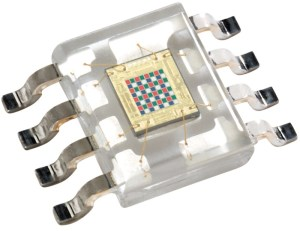
\includegraphics[scale=0.8]{images/TCS3200.jpg}
    \caption{Внешний вид микросхемы TCS3200}\label{clrsens}
\end{figure}

Внутрення структура микросхемы TCS3200 представлена на рис.~\ref{clrsensblock}. Ток с фотодиодной матрицы поступает на преобразователь ток-частота. Выход преобразователя подключен к выходному пину OUT.

\begin{figure}[H]
    \centering
    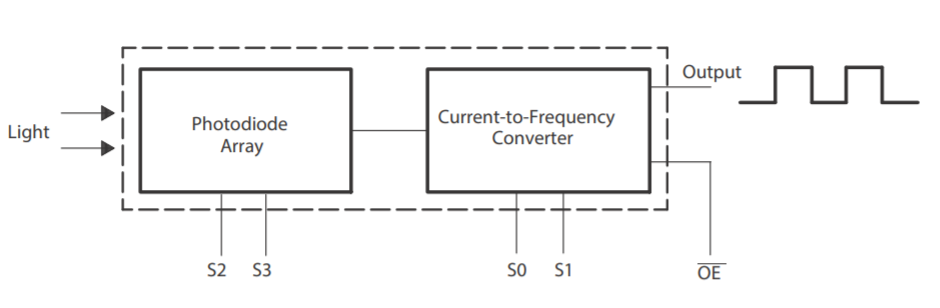
\includegraphics[scale=0.7]{images/TCS3200_block.png}
    \caption{Структурная схема микросхемы TCS3200}\label{clrsensblock}
\end{figure}

Такая внутренняя компоновка микросхемы TCS3200 позволяет датчику измерять интенсивность цвета в четырех цветовых диапазонах: синем, зеленом, красном и белом. Управлять работой датчика можно сигналами S0, S1, S2, S3 и S4 (рис.~\ref{clrsensPin}) (\textit{не путать с сигналами генератора логических уровней!}).

\begin{figure}[H]
    \centering
    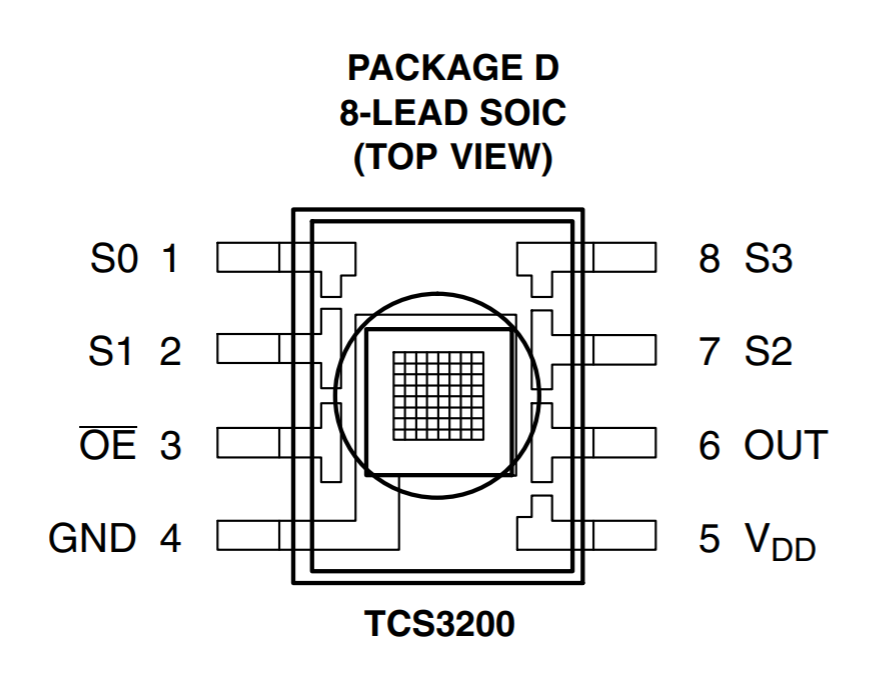
\includegraphics[scale=0.5]{images/TCS3200_pinout.png}
    \caption{Распиновка микросхемы TCS3200}\label{clrsensPin}
\end{figure}

S0/S1 позволяют выбрать диапазон выходной частоты (scaling factor), 82/83 - выбор группы фотодиодов с соответствующим светофильтром, OUT - выход последовательности импульсов с частотой, пропорциональной интенсивности цвета. Определение цвета объекта производится путем расчета отношений интенсивности (частоты), полученной от разных цветовых групп фотодиодов. Выходной сигнал датчика TCS3200 частотный. Для управления выходным сигналом необходим микроконтроллер.

К микроконтроллеру датчик цвета подключается через один разъем. Микроконтроллер должен быть запрограммирован, чтобы управлять режимами работы датчика цвета и принимать от датчика частотный сигнал. Подавая комбинацию управляющих сигналов на выводы (S2) и (S3), микроконтроллер разрешает работу датчика цвета в одном из цветовых диапазонов: синем, зеленом, красном или белом. Управляющие сигналы на выводах (S0) и (S1) задают коэффициент деления выходной частоты датчика цвета. \textit{Примечание.} в данном лабораторном комплексе выбор светофильтра датчика (измеряемого цвета) осуществляется тактовой кнопокой непосредственно возле датчика.

В модуле датчиков оба входа S0 и S1 находятся в состоянии Н. Нажатием кнопки выбора цвета управляется подача всех вариантов логических уровней на входы S2-S3. Ниже в таблице~\ref{sensoptions} приведена дешифрация состояний управляющих пинов S0-S3.

\begin{table}[H]
    \centering
    \caption{Опции датчика TCS3200}\label{sensoptions}
    \begin{tabular}{c|c|c|c|c|c}
        \toprule
        S0 & S1 & Output frequency scaling \(f_o\) & S2 & S3 & Photodiode type \\
        \midrule
        L & L & Power down & L & L & Red \\
        L & H & 2\% & L & H & Blue \\
        H & L & 20\% & H & L & Clear (no filter) \\
        H & H & 100\% & H & H & Green \\
        \bottomrule
    \end{tabular}
\end{table}

Входы S0-S1:
\begin{enumerate}
    \def\labelenumi{\arabic{enumi})}
    \item 0 - отключить выход частоты;
    \item 1 - шкала 2\% от 600 кГц максимальной возможной частоты;
    \item 2 - шкала 20\% от 600 кГц максимальной возможной частоты;
    \item 3 - шкала 100\% от 600 кГц максимальной возможной частоты (\textit{используется в данном модуле}).
\end{enumerate}

Входы S2-S3:
\begin{enumerate}
    \def\labelenumi{\arabic{enumi})}
    \item 0 - используются фотодиоды с красным фильтром;
    \item 1 - используются фотодиоды с синим фильтром;
    \item 2 - используются фотодиоды без фильтра;
    \item 3 - используются фотодиоды с зеленым фильтром.
\end{enumerate}
\textit{Примечание.} Избегайте цветовых шумов при исследовании объектов. При первом использовании модуля, при сбросе модуля или при смене источника освещения исследуемого предмета необходимо установить баланс белого.

Один из вариантов алгоритма работы микроконтроллера с датчиком:
\begin{itemize}
    \item инициализируются настройка пина внешнего прерывания, к которому подключен выход датчика;
    \item запускается разрешение на прерывания, по внешнему прерыванию считается количество импульсов сигнала \(PulseCount\) от датчика;
    \item каждый определённый промежуток времени \(Period\) прерывания глобально запрещаются и происходит подсчет частоты \(Freq\) и ее конвертация в нужное значение, а также вывод этого значения на дисплей:
    \[Freq=\frac{PulseCount}{Period},\]
    затем счётчик импульсов сбрасывается.
    \item кнопокой на модуле выбираем светофильтр датчика, снова проводим измерения;
    \item и так далее по кругу перебирая все четыре фильтра фотодиодов.
\end{itemize}

На экране дисплея отображается частота выходного сигнала в Гц для текущей настройки светофильтра датчика.

\section{Лабораторная работа}
\subsection{Цель работы}
Определить, к какой группе датчиков следует относить датчик оттенка цвета. Научиться получать правильные электрические показания с датчика, используя микроконтроллер и преобразовывать в удобную для представления человека форму (оттенок цвета).

\subsection{Оборудование}
Модуль датчиков. Модуль «Микроконтроллер ATMEGA32, компьютер/ноутбук. Измерительные цветные пластины (белого, красного, зеленого и синего цвета).

\subsection{Ход работы}
\subsubsection{Подключение}

Подключите модуль ``Микроконтроллер ATMEGA32'', модуль ``Модуль датчиков'' к внешнему блоку питания (или у портам USB компьютера/ноутбука) с помощью кабеля USB. Выполните коммутацию модулей приборными проводами в соответствии с таблицей~\ref{labtable}  и с рис.~\ref{labscheme}.

\begin{figure}[H]
    \centering
    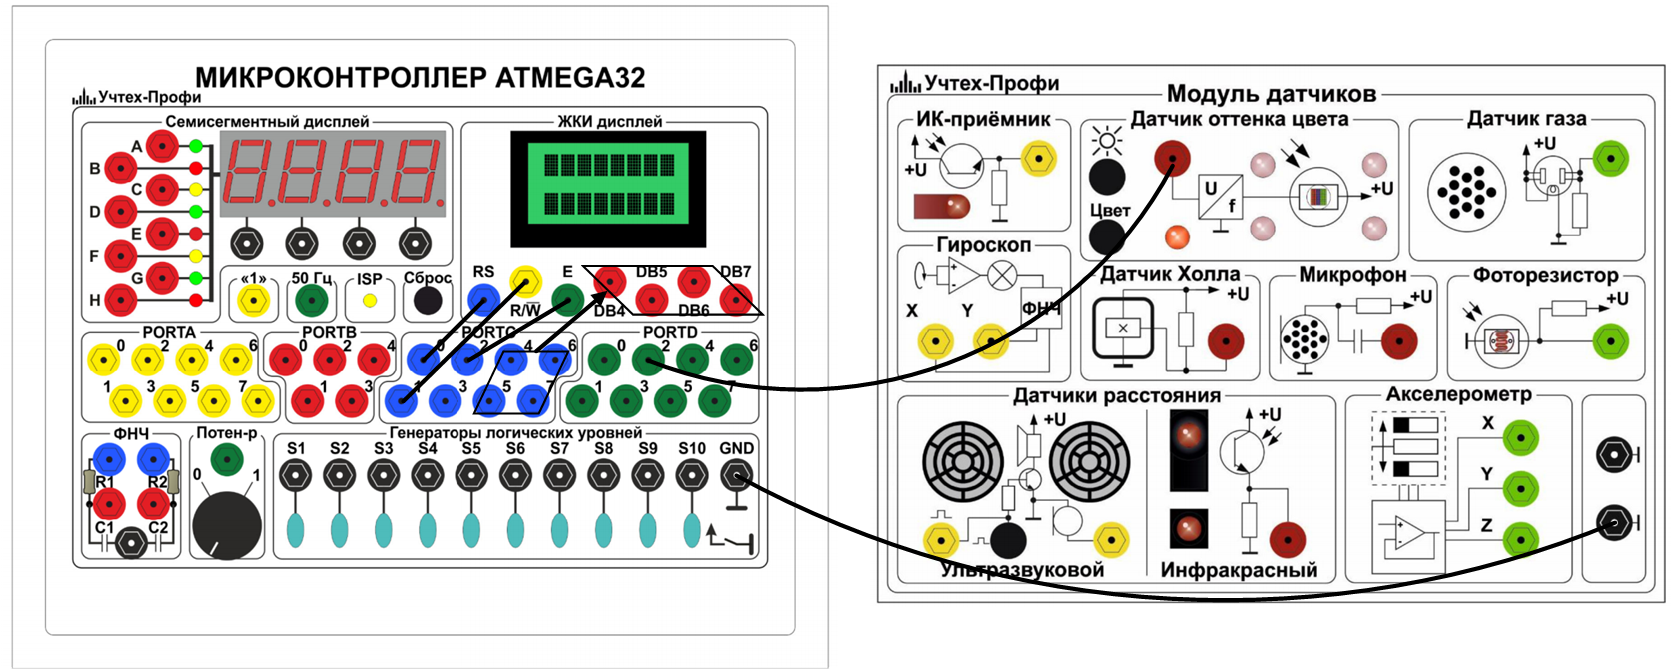
\includegraphics[scale=0.65]{images/lab2-scheme.png}
    \caption{Схема подключения модулей}\label{labscheme}
\end{figure}

\begin{table}[H]
    \caption{Коммутация модулей}\label{labtable}
    \begin{longtable}[]{@{}l|l@{}}
        \toprule
        Порт микроконтроллера ATMEGA32 & Назначение \\
        \midrule
        \endhead
        PORTC:0 & ЖК-дисплей: RS \\
        PORTC:1 & ЖК-дисплей: R/W \\
        PORTC:2 & ЖК-дисплей: E \\
        PORTC:4-7 & ЖК-дисплей: DB4-DB7 \\
        PORTD:2 & Датчик цвета \\
        \bottomrule
    \end{longtable}  
\end{table}

\subsubsection{Использование кода}

Для проведения измерений в лабораторной работе необходимо загрузить программу в микроконтроллер ATMEGA32. В папке \texttt{/src} лежат файлы исходного кода программы. Заголовочные файлы подключаемых модулей находятся \texttt{/include}. Основной выполняемый код находится в файле \texttt{/src/main.cpp}. Откройте его и проанализируйте код, который в нём содержится.

Запустите компиляцию и сборку прошивки нажав на кнопку ``Build'' на нижней панели VSCode. Затем загрузите файл прошивки в память микроконтроллера нажав на кнопку ``Upload''. После этого на ЖК-дисплее отобразятся измеряемые величины с подключённого датчика - выходная частота \(f_o\), пропорциональная интенсивности падающего света на фотодиодную матрицу микросхемы.

\subsubsection{Проведение измерений}
Необходимо провести измерения частоты выходного сигнала с датчика при разлчных светофильтрах, поднося предметы (измерительные пластины) белого, красного, синего и зеленого цвета. Пластины следует распологать на расстоянии около 5 см от датчика. 

Модуль датчика имеет две кнопки: одна включает подсветку, другая меняет тип светофильтра датчика. Выбранный светофильтр сигнализируется светодиодом возле кнопки выбора типа (если индикаторный светодиод горит белым, значит датчик настроен на измерения без светофильтра). 

\fbox{%
  \parbox{0.95\textwidth}{
    \textit{Примечание.} В модуле перепутаны красный и синий светофильтры. То есть, когда индикаторный светодиод горит красным, значит активен синий светофильтр, и наоборот, если горит синий, то активным является красный светофильтр датчика.
  }%
}

Заполните таблицу~\ref{exper} ниже. Для каждой измерительной пластины проведите измерение выходной частоты датчика \(f_o\) в Гц при всех светофильтрах. Сделайте измерения с подсветкой и без неё.

\begin{table}[H]
    \centering
    \caption{Экспериментальные измерения частоты \(f_o\), Гц}\label{exper}
    \begin{longtable}[]{c|c|c|c|c}
        \toprule
          & Без фильтра & \textcolor{red}{RED} \(f_{red}\) & \textcolor{green}{GREEN} \(f_{green}\) & \textcolor{blue}{BLUE} \(f_{blue}\) \\
        \midrule
        Белая пластина &  &  &  &  \\
        \hline
        С подсветкой: & - & - & - & - \\
        Без подсветки: & - & - & - & - \\
        \hline
        \textcolor{red}{Красная} пластина &  &  &  &  \\
        \hline
        С подсветкой: & - & - & - & - \\
        Без подсветки: & - & - & - & - \\
        \hline
        \textcolor{green}{Зеленая} пластина &  &  &  &  \\
        \hline
        С подсветкой: & - & - & - & - \\
        Без подсветки: & - & - & - & - \\
        \hline
        \textcolor{blue}{Синяя} пластина &  &  &  &  \\
        \hline
        С подсветкой: & - & - & - & - \\
        Без подсветки: & - & - & - & - \\
        \bottomrule
    \end{longtable}
\end{table}

Проанализиуйте сделанные измерения. Оценить разность показаний датчика с подсветкой и без неё.

Переведите значения частот в цветовую модель RGB 0\dots255. Для каждой цветного предмета нормируйте экспериментально полученные значения частот следующим образом:
\[RGB_{RED}=\frac{f_{red}}{\sqrt{f_{red}^2+f_{green}^2+f_{blue}^2}}\cdot255\]
\[RGB_{GREEN}=\frac{f_{green}}{\sqrt{f_{red}^2+f_{green}^2+f_{blue}^2}}\cdot255\]
\[RGB_{BLUE}=\frac{f_{blue}}{\sqrt{f_{red}^2+f_{green}^2+f_{blue}^2}}\cdot255\]
Таким образом получим диапазоны цветов в формате кортежей RGB (\(RGB_{RED}\), \(RGB_{GREEN}\), \(RGB_{BLUE}\)). Столбец ``Без фильтра'' в рассчетах не используем. Расчётные значения занесите в таблицу~\ref{rgbtable}.

\begin{table}[H]
    \centering
    \caption{Модель RGB для исследуемых предметов}\label{rgbtable}
    \begin{longtable}[]{c|c|c|c}
        \toprule
          & \textcolor{red}{R}GB & R\textcolor{green}{G}B & RG\textcolor{blue}{B} \\
        \midrule
        Белая пластина &  &  &  \\
        \hline
        С подсветкой: & - & - & - \\
        Без подсветки: & - & - & - \\
        \hline
        \textcolor{red}{Красная} пластина &  &  &  \\
        \hline
        С подсветкой: & - & - & - \\
        Без подсветки: & - & - & - \\
        \hline
        \textcolor{green}{Зеленая} пластина &  &  &  \\
        \hline
        С подсветкой: & - & - & - \\
        Без подсветки: & - & - & - \\
        \hline
        \textcolor{blue}{Синяя} пластина &  &  &  \\
        \hline
        С подсветкой: & - & - & - \\
        Без подсветки: & - & - & - \\
        \bottomrule
    \end{longtable}
\end{table}

\subsection{Вопросы}

\begin{enumerate}
    \item Принцип работы датчика оттенков цвета.
    \item Внутренняя структура микросхемы TCS3200. Принцип измерения. Вид и харакетр выходного сигнала микросхемы. Способы управления режимами работы микросхемы TCS3200.
    \item Влияние подсветки предмета, подлежащего определению цвета, на качество измерений датчика.
\end{enumerate}

\end{document}